\chapter{Studi Literatur}

Pada bab ini, Penulis akan menguraikan hasil studi literatur dalam penyusunan
tugas akhir ini. Subbab pertama membahas simulator CARLA, yaitu perangkat lunak
yang digunakan sebagai alat simulasi. Subbab kedua menjelaskan NVIDIA Pegasus
yang akan digunakan sebagai mesin untuk menjalankan algoritma \textit{decision
    making} di lingkungan simulasi dan \textit{production}. Lalu, pada subbab ketiga
akan dibahas beberapa cara komunikasi yang dapat digunakan pada antara server
simulator CARLA dengan NVIDIA Pegasus. Terakhir, subbab keempat akan membahas
penelitian-penelitian terkait simulasi \textit{autonomous vehicle} menggunakan
CARLA.

\section{Simulator CARLA}

CARLA (\textit{Car Learning to Act}) adalah perangkat lunak sumber terbuka
(\textit{o\-pen sour\-ce}) yang memiliki tujuan utama menyimulasikan kendaraan
autonomous. CAR\-LA dibangun dari nol untuk mampu melakukan pelatihan, pembuatan
prototipe, dan validasi model kemudi otonom, termasuk persepsi dan kontrol dari
model tersebut \parencite{dos_carla}.

\begin{center}
    \begin{figure}
        %% TODO: Ubah ke gambar yang di-SS sendiri
        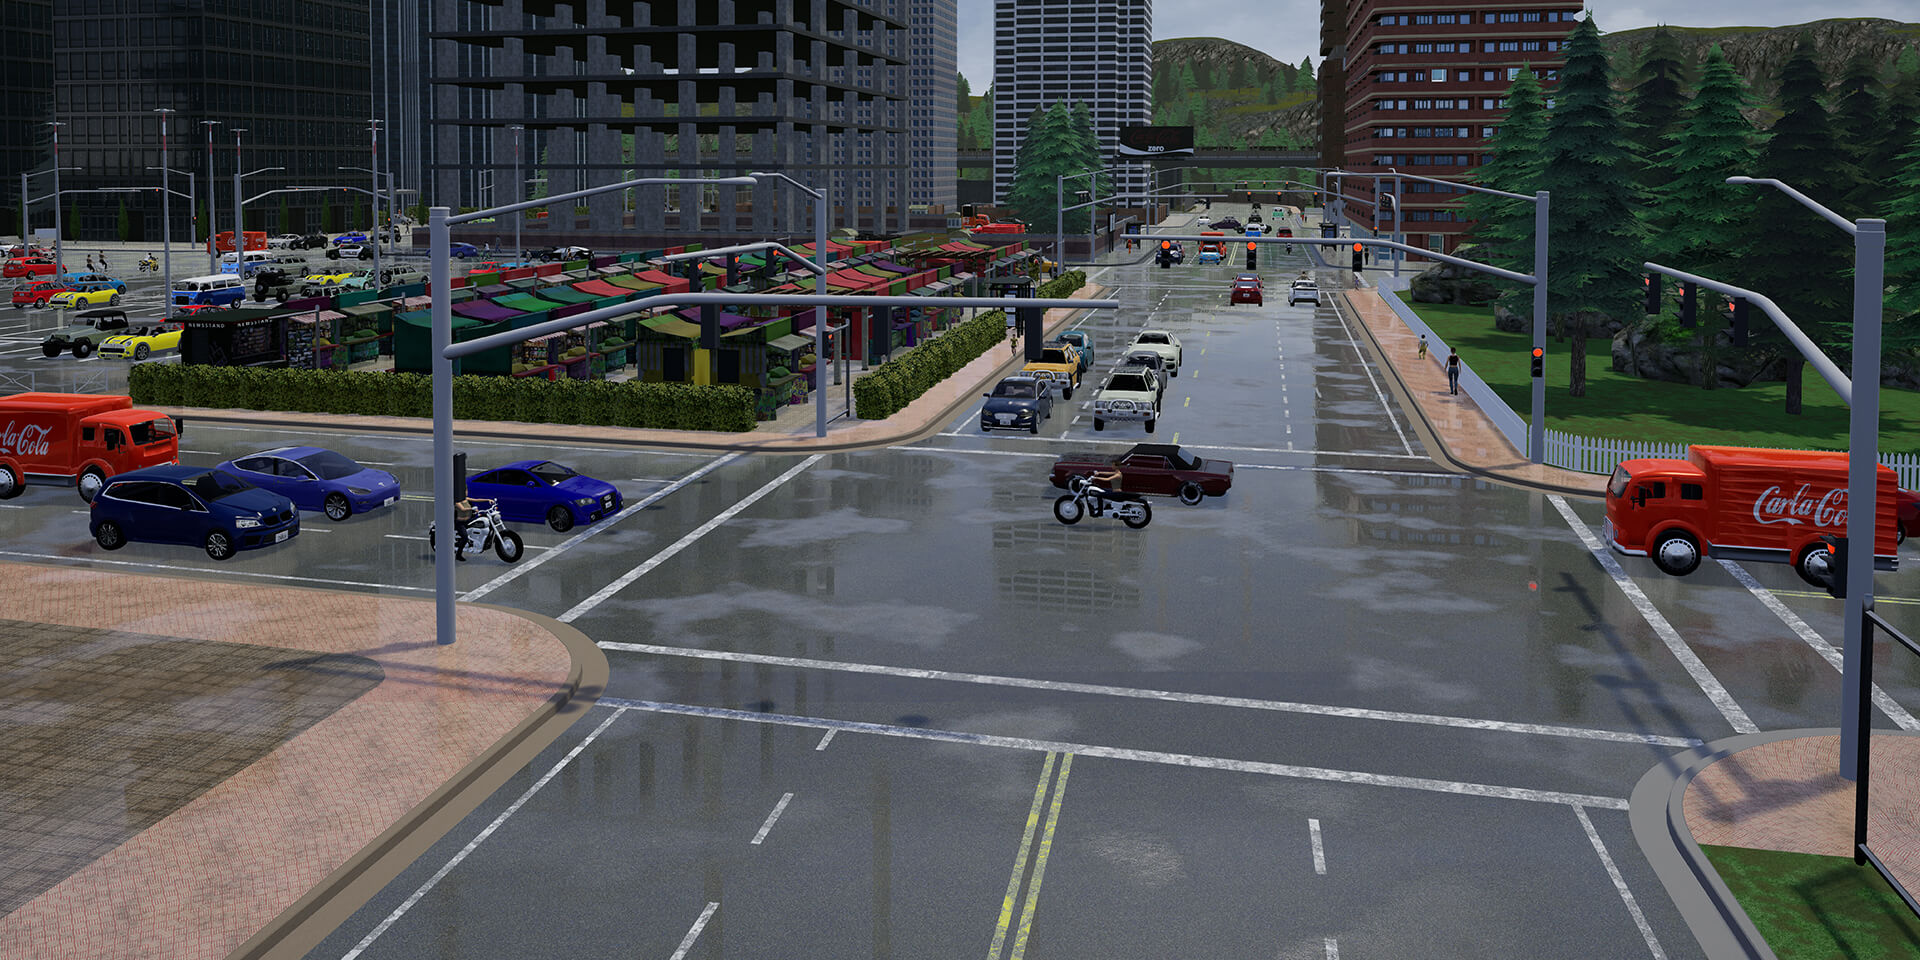
\includegraphics[width=1.0\textwidth]{resources/chapter-2/CARLA.jpg}
        \caption{Antarmuka simulator CARLA \parencite{loze_carlaDemocratizes}}
    \end{figure}
\end{center}

CARLA sendiri dibangun di atas mesin gim (\textit{game engine}) Unreal Engine 4
(UE4). UE4 dipilih karena memiliki simulasi fisika dan kualitas grafis terbaik,
setidaknya pada saat CARLA dibuat. Selain itu, UE4 juga memiliki ekosistem untuk
pengaya (\textit{plugin}) dan sistem untuk menambahkan logika dasar untuk
(\textit{non-playable character}\footnote{Istilah untuk karakter yang tidak
    dapat dimainkan pada gim.}). UE4 dan sifat sumber terbuka CARLA memungkinkan
komunitas untuk menambahkan berbagai hal sesuai dengan kebutuhan mereka atau
bahkan memperbaiki CARLA.

Agar simulasi yang dilakukan CARLA serealistis mungkin, CARLA menyediakan
berbagai macam model 3D: kendaraan, pejalan kaki, gedung, dan rambu lalu lintas.
Model-model 3D yang disediakan dibuat dengan menggunakan teknik yang
menghasilkan bentuk dan tekstur senyata mungkin, akan tetapi tetap cepat untuk
di-\textit{render}. Model kendaraan dan pejalan kaki yang dibuat bisa memiliki
banyak variasi, misalnya kendaraan Yamaha YZF dengan warna yang berbeda atau
pejalan kaki dengan aksesoris dan pakaian yang berbeda. Model-model 3D
digunakan untuk membangun lingkungan simulasi yang realistis.

Selain dari model 3D, lingkungan simulasi yang realistis didapatkan juga dari
cuaca dan waktu hari. Cuaca dan waktu hari pada CARLA dapat dikustomisasi
se\-de\-mi\-ki\-an rupa untuk memungkinkan berbagai macam skenario simulasi.
Selain itu, NPC yang ada di CARLA akan menggunakan sebuah model dari kendaraan
ataupun pejalan kaki. NPC bergerak berdasarkan suatu aturan yang sudah
ditentukan, misalnya mengikuti suatu pemilihan keputusan ketika di lampu lalu
lintas.

Selain model, CARLA juga menyediakan berbagai sensor untuk menyimulasikan
pengambilan data. Sensor-sensor tersebut dapat ``ditempelkan'' ke kendaraan
simulasi. Contoh sensor yang tersedia adalah kamera dan LIDAR (\textit{Light
    Detection and Ranging}), dan lain-lain. Selain data dari sensor, bisa didapatkan
juga data seperti kecepatan dan percepatan (mirip dengan data dari GPS) dari
kendaraan.

CARLA bekerja dengan arsitektur server-klien. Arsitektur ini memungkinkan dunia
yang dinamis dan antarmuka yang sederhana antara dunia dan agen yang
berinteraksi dengannya. Server pada CARLA berfungsi untuk menjalankan simulasi
dan me-\textit{render scene}-nya. Lalu, klien bertugas untuk mengirimkan
perintah dan ``perintah meta'' ke server dan menerima data sensor. Perintah yang
dapat dikirimkan klien digunakan untuk mengendalikan kendaraan yang
disimulasikan. Sedangkan ``perintah meta'' digunakan untuk mengatur lingkungan
simulasi, misalnya cuaca, sensor yang digunakan, dan jumlah kendaraan/pejalan
kaki NPC.

Pada sistem simulasi TA ini, komponen klien dan server CARLA akan dijalankan
pada sebuah server simulasi. Data yang didapatkan dari CARLA akan dikirim ke
sebuah server komputasi yang menggunakan NVIDIA Pegasus.

\section{NVIDIA Pegasus}

NVIDIA Pegasus adalah salah satu produk cetusan NVIDIA Corporation di bawah lini
produk NVIDIA Drive PX. Nama pasar dari NVIDIA Pegasus adalah N\-VI\-DI\-A Drive
PX Pegasus. Lini produk NVIDIA Drive sendiri merupakan platform komputer untuk
memberikan fungsionalitas bantuan mengemudi pada kendaraan bermotor.

\begin{figure}
    \begin{center}
        %% TODO: Foto sendiri (?)
        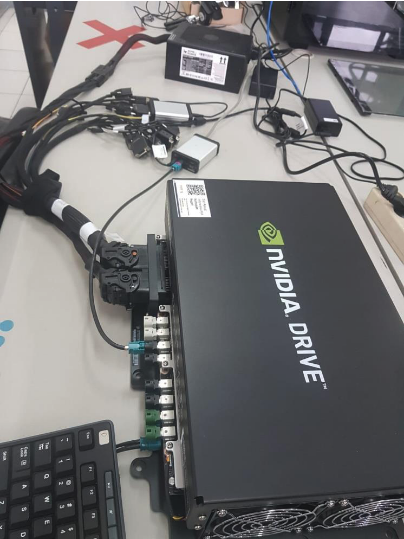
\includegraphics[width=\textwidth]{resources/chapter-2/pegasus.png}
        \caption{NVIDIA Pegasus \parencite{trilaksono_laporanRispro}}
    \end{center}
\end{figure}

Mengutip dari \parencite{oh_2017}, NVIDIA Pegasus adalah komputer yang mendukung
pengemudian \textit{autonomous} secara penuh. Artinya, NVIDIA Pegasus dapat
digunakan untuk membuat sebuah kendaraan bermotor menjadi \textit{autonomous
    vehcile} jika sensor dan algoritma yang digunakan tepat.

NVIDIA Pegasus menggunakan 2 GPU dengan arsitektur post-Volta dan 2 SoC NVIDIA
Xavier. Kombinasi CPU dan GPU ini dapat menghasilkan 320 TOPS (\textit{trillion
    operations/second}) untuk komputasi intelegensi buatan. Untuk koneksi I/O,
NVIDIA Pegasus mendukung sampai dengan 16 kamera (6 di antaranya adalah lidar).

Pada sistem simulasi yang dibuat, NVDIA Pegasus akan menjadi server yang
ber\-tang\-gung jawab atas komputasi serta \textit{decision making}. NVIDIA
Pegasus yang digunakan memiliki kumpulan kakas dan pustaka untuk membangun
aplikasi robot yang disebut ROS (\textit{robot operating system}) sehingga dapat
menjadi \textit{node} ROS.

\section{Metode Komunikasi antara Simulator CARLA dan NVI\-DI\-A Pegasus}

Pada keadaan yang ada, komunikasi antara simulator CARLA dengan NVIDIA Pegasus
menggunakan perantara \textit{web service} yang berbasis HTTP 1.1. Penggunaan
HTTP 1.1 pada \textit{web service} menjadi \textit{bottleneck}/penghambat
kinerja terbesar sistem simulasi. Ketika dilakukan secara SILS (\textit{software
    in the loop simulation} tanpa NVIDIA Pegasus) didapatkan kinerja 4000 transaksi
per detik, sedangkan ketika NVIDIA Pegasus ditambahkan ke sistem (menjadi HILS,
\textit{hardware in the loop simulation}) didapatkan 100--110 transaksi per
detik \parencite{trilaksono_laporanRispro}. Oleh karena itu, dibutuhkan protokol
atau metode komunikasi lain yang dapat meningkatkan kinerja jalur komunikasi.
Selain itu, jalur komunikasi yang digunakan harus dapat mengirimkan pesan berupa
teks \textit{string}, larik angka, atau data \textit{binary} (misalnya gambar).

\begin{figure}
    \begin{center}
        \includegraphics[width=1.0\textwidth]{resources/chapter-2/komunikasi
            data pada simulasi.png}
        \caption{Arsitektur komunikasi pada HILS
            \parencite{trilaksono_laporanRispro}}
    \end{center}
\end{figure}

Beberapa alternatif metode jalur komunikasi dapat digunakan untuk
meng\-hu\-bung\-kan kedua server akan dibahas pada subbab ini. metode tersebut
adalah komunikasi berorientasi pesan dan RPC.

\subsection{RPC}

RPC, atau \textit{remote procedure call}, secara teknis bukanlah protokol,
melainkan sebuah mekanisme untuk menyusun sistem terdistribusi yang
berkomunikasi dengan pola \textit{request/reply}
\parencite{larry_computerNetwork}. RPC memberikan abstraksi kepada pengembang
berupa pemanggilan fungsi secara lokal maupun \textit{remote}, di permukaannya,
memiliki perilaku yang sama. Pemanggilan fungsi \textit{remote} artinya
implementasi fungsi berada di komputer lain di dalam jaringan.

Ketika menggunakan RPC, pengembang tidak perlu tahu pemanggilan sebuah fung\-si
dilakukan secara lokal atau \textit{remote}; pengembang hanya perlu tahu
pemanggilan fungsi tersebut akan menghasilkan suatu nilai baru dan akan membuat
program \textit{blocking} (menunggu) sampai nilai baru tersebut
didapatkan\footnote{terdapat variasi RPC, \textit{asynchronous} RPC, yang
    memungkinkan pemanggilan fungsi \textit{remote} tanpa menghasilkan
    \textit{return} sehingga tidak perlu ditunggu.}.

Implementasi RPC yang akan dibahas pada subbab ini adalah Apache Thrift.
Apa\-che Thrift juga merupakan implementasi RPC yang akan digunakan untuk
membangun jalur komunikasi antara server NVIDIA Pegasus dengan server simulator
CARLA. Apache Thrift dipilih karena kemampuannya mengirimkan pesan dalam format
\textit{binary}. Selain itu, karena kinerja Apache Thrift lebih baik
dibandingkan dengan HTTP dan implementasi RPC oleh Google, gRPC
\parencite{abernethy_buildingHighPerformanceMSThrift}.

\subsubsection{Apache Thrift}

Apache Thrift adalah sebuah implementasi RPC dalam bentuk \textit{framework}
yang diciptakan oleh Facebook, Inc. (sekarang Meta Platforms, Inc.) lalu
disumbangkan ke Apache Software Foundation. Tujuan utama dari pembuatan Apache
Thrift adalah sebuah jembatan antar-bahasa pemrograman yang memiliki kinerja
tinggi \parencite{agarwal_thrift} sehingga Apache Thrift dapat digunakan lintas
bahasa pemrograman.

Apache Thrift memiliki beberapa abstraksi dan kakas yang memudahkan pengembang
untuk menggunakan RPC. Abstraksi-abstraksi tersebut adalah sistem tipe, protokol
(untuk \textit{encoding} pesan), transpor, pemberian versi, dan prosesor.

Abstraksi yang diberikan oleh Apache Thrift memudahkan penggunanya dalam
me\-la\-ku\-kan pengembangan sebuah layanan menggunakan RPC. Pengguna Apache
Thrift tidak perlu memikirkan cara melakukan RPC, melainkan hanya perlu
men\-de\-fi\-ni\-si\-kan layanan-layanan yang diberikan serta struktur data
tambahan pada sebuah berkas Thrift IDL (\textit{interface definition language}).
Dari definisi pada IDL tersebut, pembangkit kode Thrift (Thrift \textit{code
    generator}) akan membuat \textit{interface} untuk server dan klien. Pengguna
Thrift hanya perlu mengimplementasikan layanan-layanan tersebut pada sisi
server, sedangkan urusan protokol, transpor, dan menangani pemanggilan RPC dapat
menggunakan kakas dari pustaka Apache Thrift.

Dengan menggunakan kakas bawaan dari pustaka Thrift, pesan \textit{request} yang
di\-ki\-rim\-kan melalui lapisan transpor Thrift dapat berupa \textit{binary},
JSON, dan bentuk yang mudah dibaca manusia. Lalu, transpor yang didukung pustaka
bawaan Thrift adalah transpor menggunakan memori, berkas, HTTP, dan
\textit{socket} (TCP). Pustaka Thrift juga menyediakan transpor yang melakukan
kompresi dan transpor yang membagi pesan menjadi beberapa \textit{frame}. Jenis
server yang disediakan oleh pustaka bawaan Thrift pun beragam. Server bisa
menggunakan 1 \textit{thread} ataupun banyak \textit{thread} dengan I/O
\textit{blocking} maupun non-\textit{blocking}.

\subsection{Komunikasi Berorientasi Pesan}

Komunikasi berorientasi pesan adalah salah satu metode komunikasi pada sistem
terdistribusi. Metode ini utamanya bersifat
\textit{asynchronous}\footnote{Beberapa implementasi bisa \textit{synchronous}
    juga.}, artinya konsumen/klien tidak perlu \textit{blocking} ketika membuat
\textit{request}. Sifat \textit{asynchronous} ini merupakan alternatif untuk
serta cara berkomunikasi \textit{request/response} lainnya dan berguna ketika
konsumen tidak membutuhkan hasil pemrosesan pesan.

Implementasi untuk komunikasi berorientasi pesan yang akan dibahas adalah
protokol rosbridge dan pustaka ZeroMQ. Kedua protokol juga akan digunakan untuk
membuat jalur komunikasi antara server NVIDIA Pegasus dengan server simulator
CARLA.

% TODO: ganti jadi ROS aja
\subsubsection{Rosbridge}

Rosbridge adalah protokol komunikasi yang menambahkan antarmuka ke aplika\-si
non-ROS agar dapat berkomunikasi dengan \textit{node} ROS. Komunikasi dapat
dilakukan dengan pola \textit{publish/subscribe} ke suatu topik ROS. Dengan pola
\textit{publish/subscribe}, ROS dapat melakukan komunikasi \textit{one-to-one},
\textit{one-to-many}, \textit{many-to-one}, \textit{many-to-one}, dan
\textit{many-to-many}. Selain itu, komunikasi dapat dilakukan juga dengan pola
\textit{request/reply} dengan memanggil \textit{service} ROS.

Protokol rosbridge menggunakan format JSON untuk pesannya. Pesan yang valid
harus mengandung \textit{field} \texttt{"op"}. \textit{Field} tersebut digunakan
untuk menentukan jenis pesan. Pesan juga dapat mengandung \textit{field}
\texttt{"id"} yang digunakan sebagai penanda transaksi atau keterhubungan antara
beberapa pesan. Selain kedua \textit{field} tersebut, pesan rosbridge juga dapat
mengandung \textit{field} lainnya tergantung jenis \texttt{op}.

Secara arsitektur, rosbridge menggunakan WebSocket sebagai layanan
trans\-por\-nya. Artinya, pesan pada rosbridge pasti akan sampai dengan urutan
yang benar. Selain itu, pesan yang dikirim dapat berupa \textit{string} maupun
\textit{binary}. Pesan yang berupa \textit{string} adalah pesan dalam format
\textit{raw} JSON. Sedangkan dalam rupa \textit{binary}, rosbridge mendukung
kompresi dan \textit{encoding} dengan CBOR (\textit{concise binary object
    representation}) dan CBOR-\textit{raw}. Pesan CBOR harus didekompresi oleh
penerima menjadi \textit{raw} JSON.

Perbedaan antara CBOR dengan CBOR-\textit{raw} adalah format pesannya. Pada
CBOR-\textit{raw}, pesan dikirim dalam format serialisasi ROS. Keuntungan
menggunakan C\-B\-O\-R-\textit{raw} adalah peningkatan kinerja jika \textit{parsing}
hanya sebagian pesan, aplikasi dapat membaca berkas \texttt{bag}, atau
\textit{parsing} pesan ingin dilakukan seterlambat mungkin atau secara paralel.

\subsubsection{ZeroMQ}

ZeroMQ (\textit{zero message queue}) adalah sebuah pustaka yang merupakan
pe\-ning\-ka\-tan di atas \textit{socket} tradisional. ZeroMQ memberikan
fungsionalitas tambahan terhadap \textit{socket} dan mengabstraksi pembuatan
koneksi TCP dengan harapan memudahkan pengembangan aplikasi terdistribusi.
Fungsionalitas yang ditambahkan oleh ZeroMQ didasarkan pada pola-pola komunikasi
yang sering terjadi ketika menggunakan protokol TCP.

ZeroMQ memungkinkan komunikasi \textit{one-to-one} (seperti \textit{socket}
biasa), \textit{many-to-one} (\textit{socket} mendengarkan ke beberapa
\textit{port}), dan \textit{one-to-many}. Pola komunikasi yang didukung oleh
ZeroMQ adalah \textit{request-reply}, \textit{publish-subscribe}, dan
\textit{pipeline}. ZeroMQ juga memiliki sebuah antrian pesan (\textit{message
    queue}) sehingga pesan yang dikirimkan ke konsumen akan disimpan
sampai konsumen siap menerima pesan.

ZeroMQ berjalan di atas lapisan transpor ZMTP (ZeroMQ \textit{message transport
    protocol}). Semantik ZMTP memastikan pesan tidak akan diterima lebih dari 1 kali
oleh konsumen dan semua pesan akan diterima oleh konsumen dengan urutan yang
benar. Selain itu, \textit{frame} pesan yang diterima konsumen akan
di-\textit{queue} di memori penerima sampai semua \textit{frame} diterima.
Semantik ZMTP juga memastikan \textit{socket} dapat membuat dan menerima koneksi
serta \textit{socket} akan menyambungkan kembali jika koneksi terputus.

\section{Penelitian Terkait}

Terdapat sebuah penelitian yang memiliki lingkup serta lingkungan sama dengan
tugas akhir ini. Penelitian tersebut juga menggunakan CARLA untuk HILS.

\subsection{\textit{Hardware-in-the-Loop Autonomous Driving Simulation Without
        Real-Time Constraints}}

Pada penelitian ini \parencite{brogle_CarlaHILS}, dilakukan HILS menggunakan
NVIDIA Jetson TX1 sebagai perangkat keras untuk komputasi dan simulasi
menggunakan simulator CARLA. Salah satu hasil dari penelitian ini adalah
integrasi antara simulator CARLA dengan kakas ROS.

Arsitektur untuk menggunakan ROS dalam simulasi HILS dapat dilihat pada gambar
\ref{chapter-2-carla-jetson-arch}. Terdapat sebuah \textit{node}  yang
bertugas mendapatkan data kamera dan LiDAR dari CARLA. Kemudian, data tersebut
dipublikasikan ke topik yang didengarkan oleh pemroses data LiDAR dan vidio.
\textit{Node} yang terhubung dengan CARLA akan dikirimkan data terkait kendali
kendaraan oleh \textit{node} yang disebut \textit{path planning node}.

\begin{figure}
    \begin{center}
        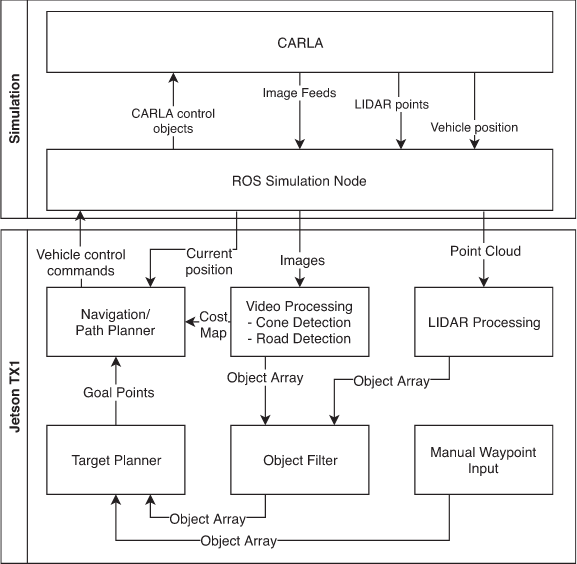
\includegraphics[width=1.0\textwidth]{resources/chapter-2/carla-jetson-arch.png}
        \caption{Arsitektur sistem simulasi \parencite{brogle_CarlaHILS}}
        \label{chapter-2-carla-jetson-arch}
    \end{center}
\end{figure}

Hasil eksperimen pada penelitian ini adalah hasil simulasi menggunakan HILS dan
CARLA tidak berbeda jauh dengan keadaan dunia nyata. Selain itu, didapatkan juga
waktu respons pada sistem simulasi lebih cepat dari dunia nyata. Sehingga, dapat
disimpulkan bahwa simulasi HILS dapat dilakukan dan implementasi dengan
menggunakan ROS (tanpa rosbridge) sudah memberikan hasil yang baik.
